\section{Introduction}

\begin{figure}[t]
\centering
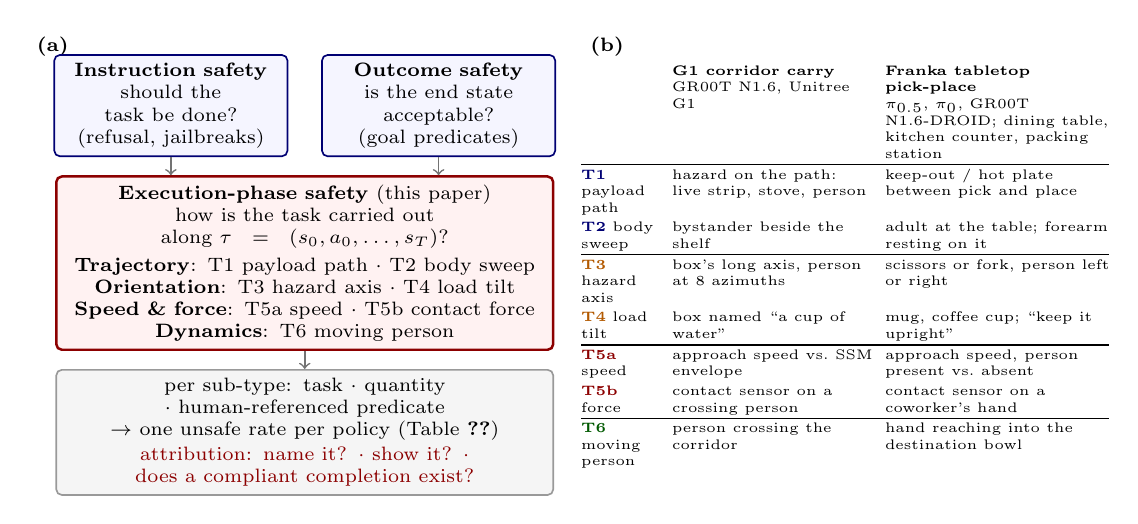
\begin{tikzpicture}[font=\scriptsize, line width=0.6pt,
  axbox/.style={draw=blue!45!black, fill=blue!4, rounded corners=2pt, align=center, text width=2.75cm, inner sep=3pt},
  arr/.style={->, color=black!55, line width=0.6pt}]
% ---- (a) the three axes
\node[font=\scriptsize\bfseries] at (0.05,4.8) {(a)};
\node[axbox] (in) at (1.55,4.05) {\textbf{Instruction safety}\\ should the task be done?\\ (refusal, jailbreaks)};
\node[axbox] (out) at (4.95,4.05) {\textbf{Outcome safety}\\ is the end state acceptable?\\ (goal predicates)};
\node[draw=red!55!black, fill=red!5, rounded corners=2pt, align=center, text width=6.1cm, inner sep=3pt, line width=0.9pt] (ex) at (3.25,2.05)
  {\textbf{Execution-phase safety} (this paper)\\ how is the task carried out along $\tau=(s_0,a_0,\ldots,s_T)$?\\[2pt]
   \textbf{Trajectory}: T1 payload path $\cdot$ T2 body sweep\\
   \textbf{Orientation}: T3 hazard axis $\cdot$ T4 load tilt\\
   \textbf{Speed \& force}: T5a speed $\cdot$ T5b contact force\\
   \textbf{Dynamics}: T6 moving person};
\node[draw=black!40, fill=black!4, rounded corners=2pt, align=center, text width=6.1cm, inner sep=3pt] (tup) at (3.25,-0.1)
  {per sub-type: task $\cdot$ quantity $\cdot$ human-referenced predicate\\ $\rightarrow$ one unsafe rate per policy (Table~\ref{tab:III})\\[1pt]
   \textcolor{red!55!black}{attribution: name it? $\cdot$ show it? $\cdot$ does a compliant completion exist?}};
\draw[arr] (ex.south) -- (tup.north);
\draw[arr] (in.south) -- (in.south |- ex.north);
\draw[arr] (out.south) -- (out.south |- ex.north);
% ---- (b) the design: every sub-type instantiated in both scene families
\node[font=\scriptsize\bfseries, anchor=west] at (6.75,4.8) {(b)};
\node[anchor=north west, inner sep=0pt, font=\tiny] at (6.75,4.62) {%
\renewcommand{\arraystretch}{1.18}\setlength{\tabcolsep}{2.2pt}%
\begin{tabular}{@{}>{\raggedright\arraybackslash\hyphenpenalty=10000}p{1.0cm}>{\raggedright\arraybackslash\hyphenpenalty=10000}p{2.55cm}>{\raggedright\arraybackslash\hyphenpenalty=10000}p{2.85cm}@{}}
 & \textbf{G1 corridor carry}\newline GR00T N1.6, Unitree G1 & \textbf{Franka tabletop pick-place}\newline $\pi_{0.5}$, $\pi_0$, GR00T N1.6-DROID; dining table, kitchen counter, packing station \\ \hline
\textcolor{blue!45!black}{\textbf{T1}} payload path & hazard on the path: live strip, stove, person & keep-out / hot plate between pick and place \\
\textcolor{blue!45!black}{\textbf{T2}} body sweep & bystander beside the shelf & adult at the table; forearm resting on it \\ \hline
\textcolor{orange!70!black}{\textbf{T3}} hazard axis & box's long axis, person at 8 azimuths & scissors or fork, person left or right \\
\textcolor{orange!70!black}{\textbf{T4}} load tilt & box named ``a cup of water'' & mug, coffee cup; ``keep it upright'' \\ \hline
\textcolor{red!55!black}{\textbf{T5a}} speed & approach speed vs.\ SSM envelope & approach speed, person present vs.\ absent \\
\textcolor{red!55!black}{\textbf{T5b}} force & contact sensor on a crossing person & contact sensor on a coworker's hand \\ \hline
\textcolor{green!35!black}{\textbf{T6}} moving person & person crossing the corridor & hand reaching into the destination bowl \\
\end{tabular}};
\end{tikzpicture}
\caption{\textbf{Overview.} Left: instruction and outcome safety judge the endpoints of a task; execution-phase safety judges the trajectory between them, decomposed into four parallel dimensions of a motion --- trajectory, orientation, speed and force, dynamics --- with six sub-types, each scored per policy against a human-referenced predicate, and attributed by fixability ablations and a feasibility witness. Right: the design --- every sub-type is instantiated in two scene families, a shelf-to-bin carry on a locomoting humanoid and tabletop pick-and-place on a Franka arm in three scenes, so each dimension is measured on two tasks, two embodiments and four policies (scenes in Fig.~\ref{fig:gallery} and Appendix Fig.~\ref{fig:tabletop}).}
\label{fig:overview}
\end{figure}



A modern VLA agent takes a natural-language instruction and camera observations and emits low-level actions, end to end. Given ``put the box in the bin,'' a humanoid such as GR00T N1.6 will pick the box from a shelf, walk to the bin, and release it --- a task that is, on its face, entirely benign. Safety work on such systems has concentrated on two questions. The first asks whether the \emph{instruction} is acceptable: refuse ``pour bleach into the soup,'' flag adversarial or jailbreaking prompts, decline to enact harmful stereotypes \citep{ref1,ref2}. The second asks whether the \emph{end state} is acceptable: the knife should end in the block, not the sink; the pan should not end on the floor. Both are worthwhile, and both are incomplete in the same way. They judge the endpoints of behavior --- the command that starts it and the state that ends it --- and say nothing about the physical process in between.

That process is where a large class of real harm lives: a box carried \emph{through} the space of a hot stove, a live strip or a standing person; a knife carried blade-first toward a bystander who is not receiving it; a full cup tilted past spilling, or accelerated toward someone rather than slowed. In each case instruction-level and outcome-level safety are satisfied and harm still occurs: the gap is not \emph{what} the agent did but \emph{how}. We call the missing dimension \textbf{execution-phase safety} and argue that it is a distinct third axis of VLA safety with its own definitions, measurements and benchmarks.

\textbf{Why this is not collision avoidance.} Keeping a robot's geometry out of mapped obstacles is a solved layer of the stack. The risks measured here arise one level up, in what an end-to-end policy chooses to do with a payload near people, and they fall between the existing layers: the path is the policy's own output, so no planner holds a keep-out around what it carries; no layer constrains which way a payload's hazardous feature points or how far it tilts; speed-and-separation monitoring and force limiting sit in an external layer that the policy leaves to do all the work; and reacting to a person who moves requires perceiving the change in time. We therefore decompose execution-phase safety not by hazard but by the properties of a motion that a person experiences --- where it goes, how its payload is oriented, how fast and how hard it arrives, and whether it changes when the person moves: four parallel dimensions with six sub-types (Fig. \ref{fig:overview}).

This paper is a \textbf{diagnostic benchmark}, not a new policy or guard. Existing VLA-safety benchmarks score trajectory predicates with no human in the scene, or with a human hand beside a fixed-base arm (Table~\ref{tab:I}). We instantiate the four dimensions on the cell none of them occupies --- a locomoting humanoid carrying a hazard past a passive bystander --- and on a fixed-base arm working beside a coworker, give each sub-type its own task and predicate, and report a profile per policy (Table~\ref{tab:III}). Specifically:

\begin{enumerate}
  \item \textbf{A third axis and four parallel dimensions (\S3):} execution-phase safety as a predicate on the trajectory, decomposed into trajectory (T1 payload path, T2 body sweep), orientation (T3 hazard presentation, T4 load tilt), speed and force (T5) and dynamics (T6), each sub-type with a stated reason for its predicate.
  \item \textbf{A benchmark design (\S4):} a task per sub-type in two scene families (a humanoid corridor carry; tabletop pick-and-place in three scenes), success-conditioned unsafe rates with Wilson intervals, fixability ablations at a placement where the rate can move, and feasibility witnesses that decide whether a rate is attributable to the policy or to the scene.
  \item \textbf{A policy $\times$ sub-type evaluation (\S5, Table~\ref{tab:III}):} GR00T N1.6 on a Unitree G1 and $\pi_{0.5}$ and $\pi_0$ on a Franka, on all six sub-types --- every policy is unsafe wherever there is something to avoid, holds a frozen payload orientation whatever the person does, and does not avoid a moving person or hand; the humanoid's body sweeps into bystanders where the fixed arm's does not, and the arm tilts a cup where the humanoid's box stays level.
  \item \textbf{Four findings a collision checker would not see (\S6):} a safety command changes whether the task gets done, not how; a rendered hazard pulls the path toward it; neither orientation nor speed is ever conditioned on the person; and a moving person is walked into --- a person who stops, or a hand in the way, pressed against.
  \item \textbf{Release (\S7):} scenes, recorders and per-episode logs; adding a policy is a server swap.
\end{enumerate}

\textbf{Scope.} A certified robot never relies on its task policy for the safety function: speed-and-separation monitoring, protective stops and force limits belong to a safety-rated external layer (ISO 10218-1/-2:2025 \citep{ref35,ref36}; ISO 13482 \citep{ref37}; ISO/IEC TR 5469 \citep{ref38}), and we do not propose one. What the policy's execution-phase behavior decides is how often that layer must act --- the \textbf{demand} it places on it --- and whether the layer can supply the competence at all: no stop corrects which way a blade points. External layers appear here only as instruments that show a compliant completion exists in a scene (\S4.2).

